
%%%%%%%%%%%%%%%%%%%%%%%%%%%%%%%%%%%%%%%%%%%%%%%%%%%%%%%%%%%%%%%%%%%%%%%%%%%%%%%%
%%%%%%%%%%%%%%%%%%%%%%%%%%%%%%%%%%%%%%%%%%%%%%%%%%%%%%%%%%%%%%%%%%%%%%%%%%%%%%%%
%%%%%%%%%%%%%%%%%%%%%%%%%%%%%%%%%%%%%%%%%%%%%%%%%%%%%%%%%%%%%%%%%%%%%%%%%%%%%%%%
\section{Descripção geral do problema inverso}

Seguindo Keller \cite{Keller76} dois problemas são considerados inversos 
um do outro, se a formulação de cada um deles envolve a resposta do outro;
de modo que por motivos históricos, um deles é bem conhecido e estudado,
pelo que recebe o nome de ``problema direto'', 
e o outro problema é novo e não pouco estudado pelo que é chamado ``problema inverso''.
 
\begin{example}[Raízes e polinômios:]~
\begin{description}
\item[Problema direto -] Achar as raízes $x_{z_1}$, $x_{z_2}$, ..., $x_{z_N}$, 
conhecendo os coeficientes do polinômio $p_{\VECTOR{c}}(x)$ agrupados no vetor $\VECTOR{c}$  \cite{Keller76}.
\item[Problema inverso -] Achar os coeficientes do polinômio $p_{\VECTOR{c}}(x)$ agrupados no vetor $\VECTOR{c}$, 
conhecendo que existem raízes em $x_{z_1}$, $x_{z_2}$, ..., $x_{z_N}$ \cite{Keller76}.
\end{description}
Uma representação gráfica do problema direto pode ser visto na Figura \ref{fig:inverso-diretos:direto1}
e do problema inverso na Figura \ref{fig:inverso-diretos:inverso1};
neste exemplo não temos entrada de dados, 
os coeficientes do polinômio agrupados no vetor $\VECTOR{c}$ são os parâmetros do sistema e 
os valores $x_{z_n}$ pertencem aos dados de saída.
\end{example}

\begin{example}[Avaliação vs. regressão:]~
\begin{description}
\item[Problema direto -] Achar os valores $y_1$,~ $y_2$,~ ...,~ $y_N$, 
conhecendo os coeficientes do polinômio $p_{\VECTOR{c}}(x)$ agrupados no vetor $\VECTOR{c}$ e
os valores $x_1$, $x_2$, ..., $x_N$ \cite{Keller76}.
\item[Problema inverso -] Achar os coeficientes do polinômio $p_{\VECTOR{c}}(x)$ agrupados no vetor $\VECTOR{c}$, 
conhecendo que existem os valores $x_1$, $x_2$, ..., $x_N$ e 
$y_1$,~ $y_2$,~ ...,~ $y_N$  \cite{Keller76}.
\end{description}
Uma representação gráfica do problema direto pode ser visto na Figura \ref{fig:inverso-diretos:direto1}
e do problema inverso na Figura \ref{fig:inverso-diretos:inverso1}, 
onde $x_n$ pertence à entrada de dados, 
os coeficientes do polinômio agrupados no vetor $\VECTOR{c}$ são os parâmetros do sistema e $y_n$ pertence aos dados de saída.
\end{example}


\begin{example}[Avaliação vs. regressão:]~
\begin{description}
\item[Problema direto -] Achar os valores $y_1$, $y_2$, ..., $y_n$, ..., $y_N$, 
conhecendo vários coeficientes para o polinômio $p_{\VECTOR{c}_n}(x)$ agrupados no vetores $\VECTOR{c}_n$ e
um valor $x$ \cite{Keller76}.
\item[Problema inverso -] Achar o valor $x$
conhecendo vários coeficientes para o polinômio $p_{\VECTOR{c}_n}(x)$ agrupados no vetores $\VECTOR{c}_n$ e
os valores $y_1$, $y_2$, ..., $y_n$, ..., $y_N$  \cite{Keller76}.
\end{description}
Uma representação gráfica do problema direto pode ser visto na Figura \ref{fig:inverso-diretos:direto1}
e do problema inverso na Figura \ref{fig:inverso-diretos:inverso2}.
\end{example}

\begin{figure}[!h]
     \centering
     \begin{subfigure}[b]{0.49\textwidth}
         \centering
         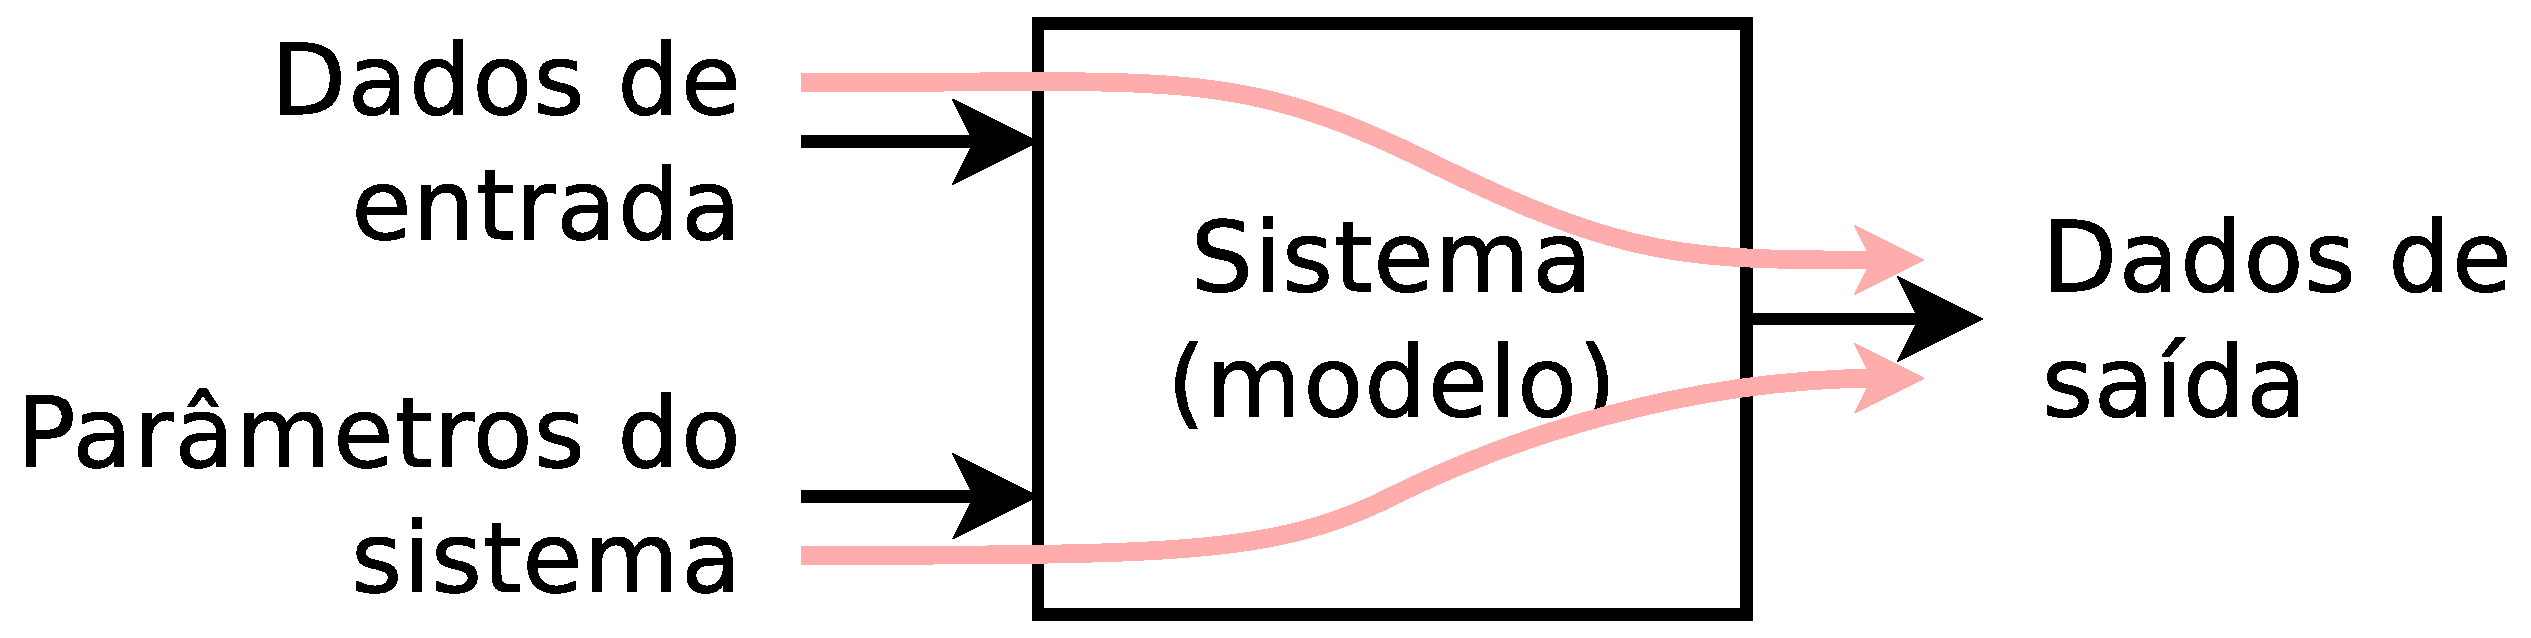
\includegraphics[width=0.95\textwidth]{chapters/notacao/direto1.eps}
         \caption{Problema direto.}
         \label{fig:inverso-diretos:direto1}
     \end{subfigure}
     \hfill
     \begin{subfigure}[b]{0.49\textwidth}
         \centering
         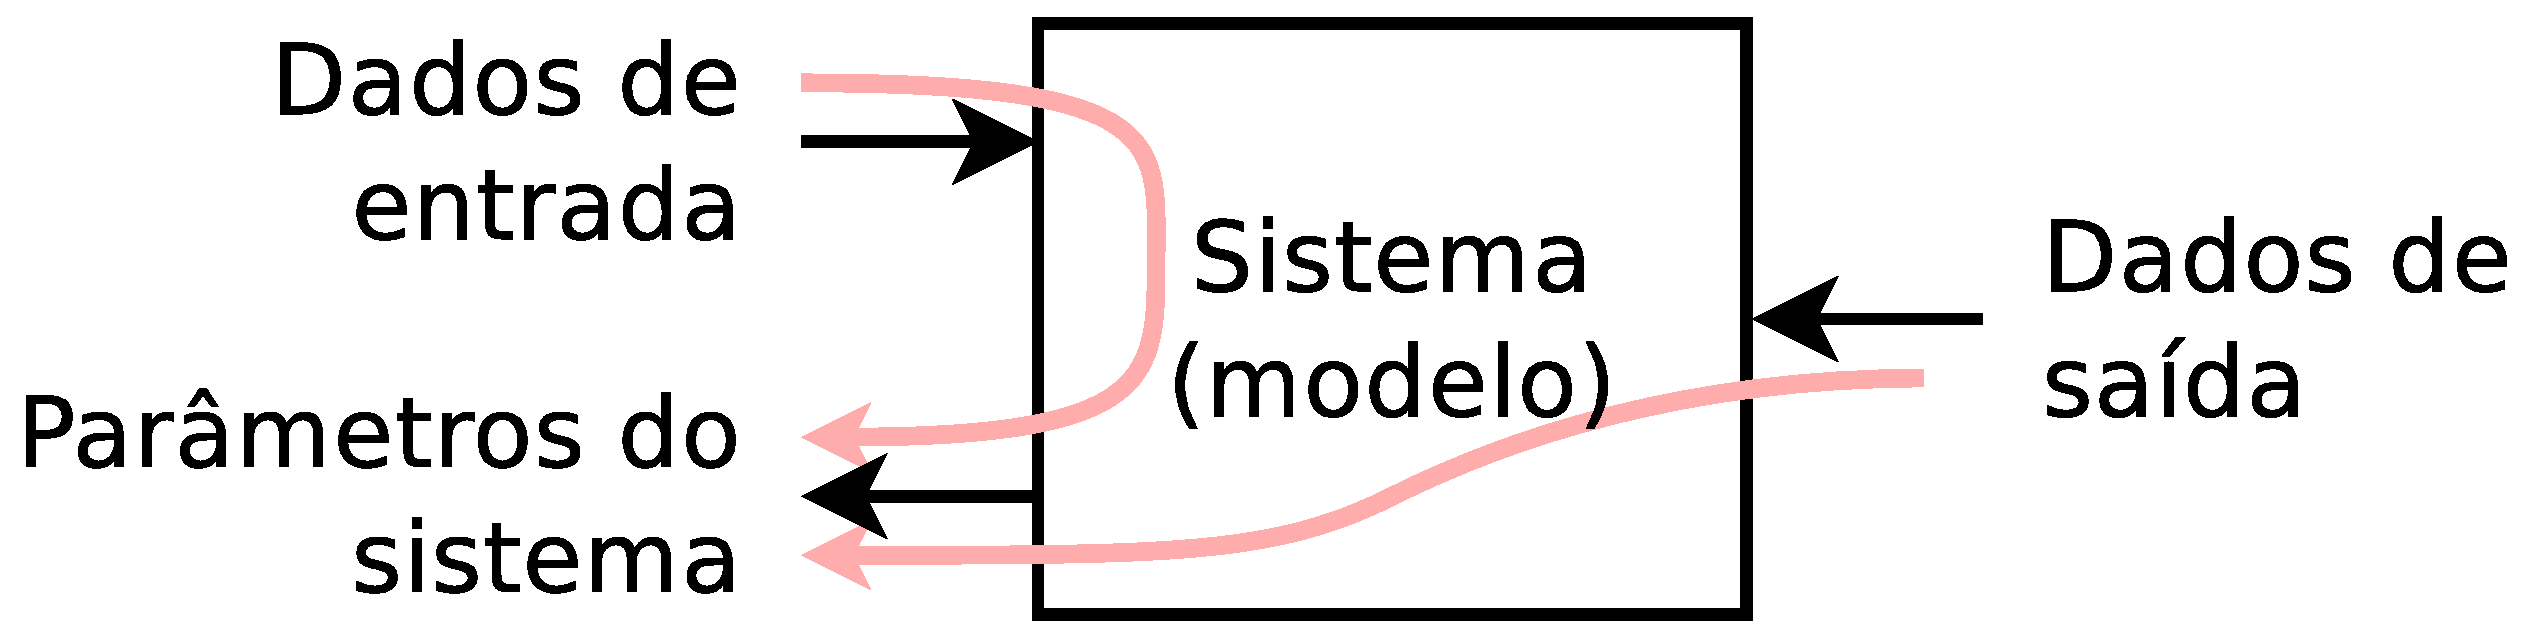
\includegraphics[width=0.95\textwidth]{chapters/notacao/inverso1.eps}
         \caption{Problema inverso.}
         \label{fig:inverso-diretos:inverso1}
     \end{subfigure}
     \hfill
     \begin{subfigure}[b]{0.49\textwidth}
         \centering
         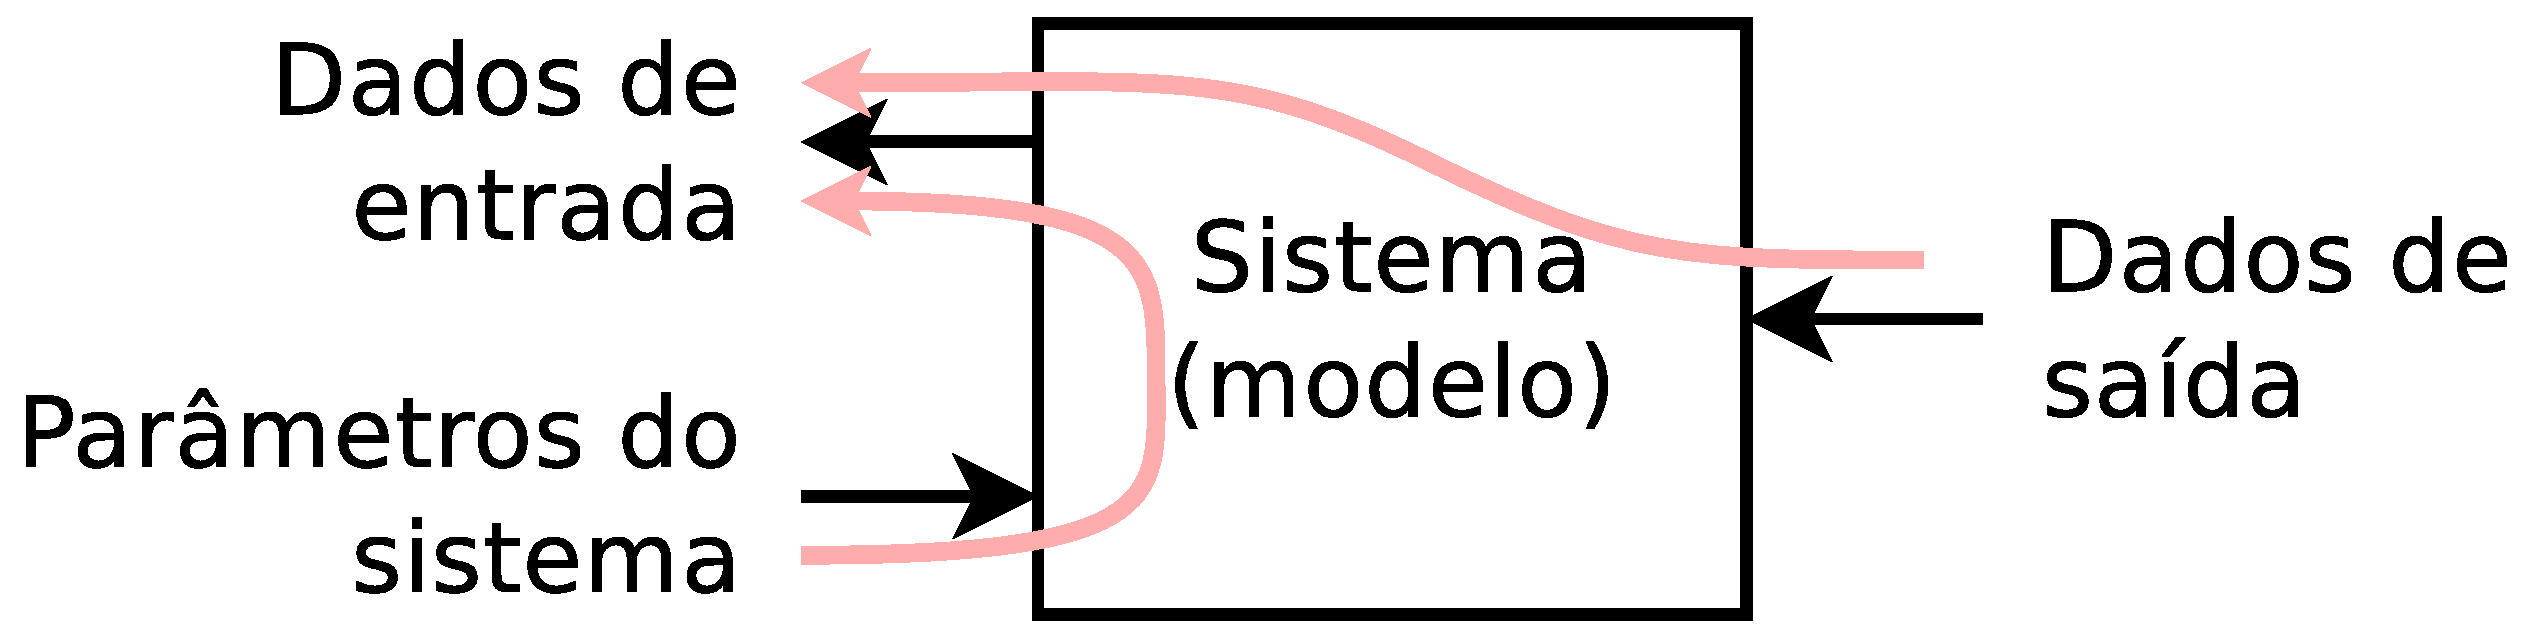
\includegraphics[width=0.95\textwidth]{chapters/notacao/inverso2.eps}
         \caption{Problema inverso.}
         \label{fig:inverso-diretos:inverso2}
     \end{subfigure}
        \caption{Exemplos de problemas diretos e inversos.}
        \label{fig:inverso-diretos}
\end{figure}

